%proofread!

%\documentclass[draft,jgrga]{agutex}
\documentclass[12pt]{article}
\usepackage[dvips]{graphicx}
\usepackage{amsmath}
\usepackage{multirow}
\usepackage{caption}
\usepackage{array}
\usepackage{natbib}
%\usepackage{authblk}

\usepackage{tabularx}
%\usepackage{lineno}
%\linenumbers*[1]

%\noindent $>$latex file \\
%\noindent $>$dvips -P pdf -o file.ps file.dvi \\
%\noindent $>$ps2pdf13 file.ps file.pdf

%\authorrunninghead{GUTOWSKI ET AL.}
%\titlerunninghead{Radar uncertainty}

\begin{document}

\title{Uncertainty of Ice-penetrating Radar and New Age-Depth Profiles at Byrd Ice Core, West Antarctica}
\author{Gail Gutowski\\ Department of Geosciences, University of Texas at Austin, Austin, TX \and Charles Jackson, Donald Blankenship, Duncan Young \\Institute for Geophysics, University of Texas at Austin, Austin, TX}
\maketitle


\begin{abstract}
%We present a new depth chronology for ice near Byrd ice core which accounts for uncertainties in ice penetrating radar and ice core dating. Our chronology consists of an ensemble of age-depth profiles representing the physical range of uncertainty associated with prominent radar reflectors in the ice. These profiles are useful for inferring ice strain rates and ice velocities, which are necessary for modeling ice dynamics.

We present estimates of age-depth relationships for prominent radar reflectors near Byrd Ice Core, West Antarctica. The estimates use a simple ice flow model and a Bayesian approach to synthesize constraints and uncertainties affecting the determination of the depth of a radar reflection horizons and ice core ages. With these prominent reflectors dates, it is possible to map the strain rate history through entire basins where depth to these reflectors have been sufficiently mapped. We find that age-depth uncertainty introduced by radar is approximately 2 m and is constantly with depth below 168 m. Combined with an assumed 3\% uncertainty in age in the ice column, we find that some pairs of spatially distinct radar horizons are consistent with being isochronous deposition events. This information is useful to determining the duration of past events affecting ice fabric, such as volcanic events. It also suggests the importance of including a complete accounting of uncertainty, including uncertainty from dating, to fully describe the dynamic evolution even in interior regions of an ice sheet.
\end{abstract}

%\begin{article}
\section{Introduction}

Ice sheet response to changes in climatic conditions in the past can be useful in evaluating future response. Age-depth relationships from ice cores are one tool available for understanding ice dynamics and accumulation history of on an ice sheet. More recently, ice-penetrating radar has made it possible to extend age-depth profiles over larger regions of the ice sheet \citep[e.g.][]{neumann2008,holt2006}.

Englacial radar horizons encode information about accumulation rates and ice deformation which can be used to determine ice velocities and strain rates. Such a picture of ice dynamics has been lacking in the past; the last report by the Intergovernmental Panel on Climate Change neglected the influence of ice dynamics in its projections of future sea level rise \citep{ipcc2007}, due to a lack of knowledge. Many modeling efforts are underway to fill this gap and will benefit from incorporation of englacial metrics for model validation.

However, it is important to understand uncertainty in ice-penetrating radar data and how that uncertainty may affect interpretation of paleo ice evolution. The accuracy of dating englacial radar horizons depends on uncertainty in radar observations and in ice-core dating. \cite{eisen2004} evaluated this uncertainty for ground-based radar in the top 100 m of the East Antarctic Ice Sheet. We approach the problem using ice-penetrating radar observations of the West Antarctic Ice Sheet (WAIS) near Byrd ice core and consider radar horizons in the upper 1300 m.  We use an ice-core derived chronology and a one-dimensional ice flow model to evaluate age and depth uncertainty of the ice using a Bayesian framework based using a Markov Chain Monte Carlo technique. We present a resulting ensemble of age-depth profiles, which represents a probabilistic picture of the relationship between age and depth at the Byrd ice core.

\section{Data}

\subsection{Radar Data}
%*See Marie's paper for language*
Ice-penetrating radar-echo sounding data was obtained in December 2004 as part of the Airborne Geophysical Survey of the Amundsen Sea Embayment (AGASEA) project \citep{holt2006}. The radar line passed 870 m from the Byrd ice core site while the plane was traveling 67 m/s at an elevation of 550 m above the ice surface. The data includes two-way travel times (the time it takes for a radar pulse to be transmitted, reflect off an englacial horizon, and return to the receiver) in microseconds, which were collected with a 15 MHz bandwidth. We use ten strong radar horizons that were traced using the seismic imaging software \textit{GeoFrame} based on peaks and troughs in the return signal. The horizons were selected for their prominence in the signal and continuity through the domain. The ten horizons of interest are shown in Figure~\ref{radargram}.
%Geoframe ref?

Radar reflection horizons provide an avenue for developing an understanding of ice dynamics. Each year, snow accumulates on the surface of the ice sheet. The physical properties of this snow contain information about climatic conditions at the time of deposition; for instance, the oxygen isotope, $\delta^{18}O$, can be used as a proxy for temperature. Over time, the surface layer is covered with the accumulation of subsequent years and becomes buried in the ice column. Differences in chemical composition of these deposited layers lead to variations in electrical conductivity observed by the radar as horizons, or horizontal layers. We therefore interpret the radar horizons as isochronous \citep{eisen2004}.

\subsection{Byrd ice core chronology}

The Byrd ice core was drilled in 1968 and was the first in Antarctica to extend to bedrock \citep{gow1968}. Damage to the ice core above 88 m prohibited the traditional approach of annual layer counting. However, in 1989 a shallow core dubbed NBY89 was drilled nearby which enabled \citep{langway1994} to complete a chronology for the top 164 m of the ice column. Below 88 m, the electrical conductivity method (ECM) was used to date the ice core \citep{hammer1994}. The ECM method measures variations in electrical conductivity. Between 300 m and 900 m, brittle ice precluded sufficient ECM measurements. \citet{hammer1994} instead fit the chronology with three piecewise linear functions. The resulting layer-thickness profile was integrated from surface to depth to obtain an age-depth relationship for the length of the ice core.

\citet{hammer1997} present a volcanic chronology based on this previously derived timescale in which volcanic events were matched to peaks in electrical conductivity. The chronology includes dated volcanic events that cover an age range from 709 BP to more than 18000 BP, corresponding to depths ranging from 97.8 m to 1890 m below the 1968 surface of the Byrd ice core. We use part of this volcanic record to 1358 m depth (corresponding to 20594 a) as an observational constraint on our age-depth profile.



\section{Sources of Uncertainty}\label{unc}
There are many sources of uncertainty inherent to the way in which
data is collected, analyzed, and understood. We have included the
following sources of uncertainty in our analysis.

\subsection{Depth Uncertainty }\label{radunc}
%See Marie's paper for language
Englacial radar horizons, surfaces of constant two-way travel time (TWTT), are traced using seismic interpretation software. The software allows users to select strong reflectors from a radargram and trace them along a radar line. However, there is a limit to the accuracy of tracking a single phase of a radar reflection. The vertical accuracy depends on the resolution of the sampling rate of the radar transmitter as well as considerations of noise. For high sampling rates, the uncertainty in phase selection is typically $\frac{\lambda}{2}$, but can be as accurate as $\frac{\lambda}{4}$ for data with high signal-to-noise where $\lambda$ is the wavelength of the electromagnetic pulse.  The sampling rate for the data used here varies from 5 ns to 20 ns. Conservatively, we assume a 10 ns resolution when tracking the phase of reflections from the surface of the ice sheet and from each englacial reflector. We treat the surface and englacial horizons separately in this instance. 

To convert TWTT uncertainty into depth uncertainty, we scale TWTT by the velocity of electromagnetic wave propagation in the mediums through which it passes, namely air between the plane and the surface and ice otherwise. We take the velocity of electromagnetic wave propagation in ice to be $\textit{c}_i$ = 1.69 x 10$^8$ m/s before reaching the internal layers and reflecting back. The corresponding 1$\sigma$ uncertainty is $\sigma_{surf}$ $\sim$0.3 m for the surface reflector and $\sigma_{lay}~\sim~$0.17 m for each of the internal layers, assuming a gaussian probability distribution.
 
The error associated with assigning the elevation of the surface is systematic because the same surface elevation will be used to normalize all of the internal layers. Conversely, the TWTT uncertainty of each of the internal layers is applied randomly, as each of the individual layers need not have the same uncertainty. This is due to the fact that reflection from each horizon need not  have the same phase with respect to the sampling rate. To account for this, we assume TWTT uncertainty to be normally distributed and sample randomly from this distribution for each of the internal layers, independent of samples for other horizons.

The finite bandwidth of the data means that even an infinitesimally thin layer of ice will appear in the survey to have a finite width. Our data uses a pulse bandwidth of 15 MHz. This translates to a 1$\sigma$ depth uncertainty of 5.63 m, obtained from considering both the bandwidth frequency and the velocity of electromagnetic radiation in ice. This uncertainty is applied as a random, normally distributed error in the depth of each of our selected layers. 

Ice density data as a function of depth were obtained from the original analysis of the ice core \citep{gow1968}. The data were used to account for the varying density of ice and subsequent variations in electromagnetic wave speed through the firn layer in the top 


\subsection{Age Uncertainty}\label{ageunc}

The ice core chronology at Byrd is uncertain due to damage in the upper part of the core, a zone is brittle ice between 788 m and 900 m depth, and subjectivity in the interpration of ECM results, among other reasons. \citet{hammer1994} suggest a precision of $\pm$ 1000 years for 20000 ka ice due to subjectivity in the ECM technique. They also give an approximate accuracy of 11000 ka ice as $\pm$ 500 years. The volcanic chronology developed by \citet{hammer1997} quotes $\pm$ 500 years for the prominent Old Faithful radar horizon observed to be approximately 17400 ka old. Due to a lack of uncertainty analysis of the ice core chronology, we assume an uncertainty distribution that is 3\% of the observed age of the ice column. For example, this assumes that Old Faithful is of age 17400 $\pm$ 522 ka and that a layer of age 10000 ka has uncertainty $\pm$ 300 yr. 

This assumed uncertainty follows the trend we expect, assigning larger uncertainty to ice deeper in the ice column where shear thinning results in layers that are more difficult to distinguish from one another and where disruptions in shallower parts of the ice core can contribute uncertainty to the dating of deeper layers. An estimate of 3\% uncertainty is in line with, though conservative compared to, expert opinion.  Without additional information for uncertainty analysis, we contend this is an appropriate first-order description of the uncertainty in Byrd ice core chronology. Synthesis of multiple dating techniques as correlation between the Byrd ice core to Greenland ice cores, such as in \citet{blunier2001} may provide an improved estimate of age uncertainty.

%Each year, fresh snow accumulates on top of the ice sheet, burying the previous season's snowfall. As layers of ice are advected into the ice sheet, they become thinner as the ice is compacted due to increasing overlying ice and shear thinning from ice flow. This thinning makes it increasingly difficult to distinguish one between horizons at depth. In shallow regions, it is possible to count layers by eye to determine the age of near-surface isochrones; however, this is harder to do deep in the ice sheet. The uncertainty associated with determining ages for ice layers is therefore a function of depth. 

%The upper part of the original 1968 Byrd ice core was too damaged to count annual layers. However, in 1989, a shallow core dubbed NBY89 was drilled nearby which enabled \citep{langway1994} to complete a chronology for the top 164 m of the core. Using the ECM method \footnote{ The Electrical Conductivity Method (ECM) is another approach to dating ice. It involves measuring the conductivity of ice at different depths \citep{hammer1994}. This conductivity is associated with the composition of the ice, characterized by its acidity level. Layers of ash embedded in the ice, for example, will have a distinct conductivity. The ECM method is particularly useful in deep parts of the ice column where it is difficult to otherwise distinguish isochronous layers due to layer thinning.}, they matched 3 volcanic events to the original ice core with an uncertainty of $\sigma_{age} = \pm$ 2 yr for the upper 1360 a of the ice core.

%Isotopic dating is common among ice core chronologies. Landmark events for concentrations of Beryllium-10, methane, and fluorine (to name a few) are matched to chemical analyses of the ice \citep{schwander2001} at different points in time. Accepted dates for these events are then mapped onto the ice core. 

%We adopt the following estimates of uncertainty to accompany the isotopic dating, though no comprehensive review of uncertainty from these methods is available. The end of the Younger Dryas period is correlated between the GRIP and Byrd ice cores using CH$_4$. This method indicates an uncertainty of roughly $\sigma_{age} = \pm$ 150 yr for the period between 1360 a and 11.5 ka \citep{ blunier1998, schwander2001}. This incorporates uncertainty in the $\delta$age estimate on the GRIP and Byrd cores ($\pm$ 100 yr) as well as the CH$_4$ match between the GRIP/Byrd ($\pm$ 100 yr). For the period between 11500 a and 17320, we adopt an uncertainty of $\sigma_{age} = \pm$ 300 yr \citep{schwander2001}. This value is the result of stratigraphic layer counting near a prominent fluoride peak at Byrd station, tuned by matching CH$_4$ during the Younger Dryas period.

%For layers older than 17320 a, we assume $\sigma_{age}$ = 2 ka based on U/Th dating of the Laschamp geomagnetic excursion \citep{schramm2000}. Note that we include this uncertainty for completeness; the ten radar horizons of interest in this analysis are believed to be younger than 17320 a.

%Table~\ref{age_unc} summarizes the uncertainty we assign to observed ages as a function of depth.


\section{Method}\label{method}

We use an ice flow model adapted from \citet{morland2009} to determine the age of internal layers near the Byrd ice core drilling site in Antarctica.  The simple flow model has the form:
\begin{equation}
\begin{array}{l}
\displaystyle \frac{\overline{z}}{h_0} = \frac{1}{1 - r} [1 - exp(-s \overline{t})]\\
\\
\displaystyle \overline{z} = h_0 - z\\
\\
\displaystyle r = \frac{b}{q}\\
\\
\displaystyle s = s_ds_0\\
\end{array}
\end{equation}
\\

where depth, $\overline{z}$, is defined to be 0 at the base, $h_0 =$ 2164 m is the depth at the ice sheet surface, b is basal melting rate, q is the accumulation rate, and $\overline{t}$ is the age corresponding to $\overline{z}$. The optimum constant strain rate, $\textit{s}$, is used to achieve reasonable correlations between the model and observations; $s_0$ is the initial strain rate and $s_d$ is determined empirically for the Byrd ice core to be $s_d$ = 0.722 for the Byrd ice core \citep{morland2009}. The model assumes isostatic equilibrium, constant ice density, uniform strain rate in $\textit{z}$, and $\textit{r}$ $<$ 1 (i.e. nonnegative mass balance in the ice column). Note that it is difficult to know accumulation rate on its own due to layer thinning within the ice column. As such, we consider layer thickness instead of layer accumulation because it can be physically measured using the techniques described previously. Further, while depth in the model, $\overline{z}$, is defined so that $\overline{z}$(base) $=$ 0, the following analysis is discussed in terms of depth $\textit{z}$, where $\textit{z(surface)} = 0$.

We use the flow model to invert for accumulation as a function of depth, $\textit{q}$, and strain scale factor, $\textit{s}$, using an observed age-depth relationship. We use the resulting parameters to evaluate the age of ten prominent radar horizons. The inversion is done using a Markov Chain Monte Carlo technique known as the Metropolis-Hastings algorithm \cite{metropolis1953}. We use a stepwise function to parameterize accumulation in four depth regimes:

$$
z = \left\{ \begin{array}{rl}
z_1 & \mbox{  z $< 150$m } \\
z_2 & \mbox{  150m $\le$ z $< 1024 m$ m} \\
z_3 & \mbox{  1024m $\le$ z $ < 1294$m} \\
z_4 & \mbox{  z $\ge$ 1292m }\end{array} \right.
\\
$$

These regimes were chosen based on a linear piecewise function of layer thickness developed by \citet{hammer1994} in which slope changes are observed at the above transition points. % For this analysis, we use the calculated strain rate to express accumulation from the model in terms of layer thickness for comparison to observations according to the simple strain thinning relationship:

%\begin{equation}
%\.{b} = s \lambda
%\end{equation}
%\\
%where $\.{b}$ is accumulation and $\lamdba$ is layer thickness which are related by the (assumed uniform) vertical strain rate.

The Metropolis algorithm utilizes prior knowledge about the model parameters (accumulation and strain scale factor) to develop a joint posterior distribution of the parameters. We use truncated uniform priors on all parameters, allowing them to take on values within a physically reasonable range: layer thickness is allowed to vary between 0 cm/a and 30 cm/a, while the strain scale factor may take values between 0 and 1.7.  The model is initialized using random parameter values within these ranges.

At each model step, we evaluate the age model at every point in the ice column based on proposed sets of parameters.  An associated cost is calculated as a measure of the model/data misfit for each proposal. The log likelihood is described in equation~\ref{cost}:

\begin{equation}\label{cost}
log likelihood = \frac{(Age_{model}~ - ~Age_{obs})^2}{(2\sigma_{obs})^2}
\end{equation}
\\

where $Age_{model}$ is evaluation of the \citet{morland2009} ice flow model for a given accumulation and strain scale factor. $Age_{obs}$ and $\sigma_{obs}$ come from the volcanic age-depth function and we allow for the aforementioned uncertainty in $Age_{obs}$ to loosen the constraint on the cost function. At each iteration the algorithm makes a decision about whether or not to accept the combination of parameters based on the cost: if the cost of the $\textit{n}$th iteration is less than the cost of the $\textit{(n-1)}$th iteration, the set of parameters is accepted. This means that the $\textit{n}$th set of parameters is a better fit to the data, because the cost has decreased. If the cost of the current nth iteration is greater than the cost of the $\textit{(n-1)}$th iteration, the set of parameters is accepted with probability $exp[-\frac{cost_n~-~cost_{n-1}}{2}]$, the Metropolis probability. The algorithm continues on a random walk through parameter space, minimizing cost at each step.

We use the Metropolis algorithm to generate a large number of age-depth distributions that together describe the probability of the age of a radar horizon at a given depth based on knowledge about ice flow and layer thickness. We generate 20000 sets of parameters (accumulation and strain rate) that characterize physically reasonable models of age-depth. Age uncertainty is taken to be the variance in age at a given depth. 

Uncertainty in the radar-derived depth of each horizon is considered next. To find the radar sampling rate uncertainties, we draw a single value from the probability distribution for the surface reflector, described by $\sigma_{surf}$. We then randomly sample ten values from a probability distribution described by $\sigma_{lay}$, resulting in a radar sampling rate for each of the horizons of interest. The bandwidth uncertainty is found in the same fashion as the sampling rate error for the layers. Total radar uncertainty for each radar horizon is taken to be the root mean square of the bandwidth and sampling rate uncertainties. We also add a correction for firn density and account for additional accumulation between 1968 (when the core was drilled) and 2004 (when the radar line was flown) assuming a constant accumulation rate of 11 cm/a \cite{hammer1994}. 

This process is repeated 20000 times to build a probability distribution describing the depth of each radar horizon. For each sample in depth probability distribution (20000 in all), we randomly sample an age-depth model from the ensemble generated previously. The selected model is evaluated at each of the ten radar horizon depths for a given sample. The result is an ensemble of 20000 age-depth profiles for the radar horizons of interest which incorporate uncertainty in both age and depth.



\section{Results}


Figure~\ref{agedepthhist}a shows the distribution of modeled depths associated with each ice layer of interest from radar observations near Byrd Station, West Antarctica. The spread in the distribution is indicative of uncertainty due to observational methods. Table~$\ref{results}$ shows the standard deviation of depth for each of the ten chosen layers, assuming the errors to be gaussian. See Section~$\ref{ageunc}$ for a full discussion of the sources of uncertainty included in this analysis. The uncertainty in each layer depth is more or less constant with depth. 

The corresponding age distributions are shown in Figure~\ref{agedepthhist}b and again assume gaussian errors. Table~\ref{results} shows the mean and standard deviation for each peak. Due to increased uncertainty in ice core dating, age uncertainty increases with depth. As Figure~\ref{agedepthhist} shows, horizons at 738.8 $\pm$ 2.3 m and 759.1 $\pm$ 2.3 m (horizons 7 and 8) are consistent within age uncertainty, indicating they may have been deposited at the same time. Similarly, horizons 9 and 10 (1257.7 $\pm$ 2.4 m and 1266.2 $\pm$ 2.3 m depth) are barely distinct in depth, but are likely isochronous when age uncertainty is included in the analysis.  This ambiguity makes it clear that robust uncertainty quantification is critical for the interpretation of internal layers; dynamic analyses require that radar horizons be distinguished in order to obtain a time-dependent profile of ice flow. 

Figure~$\ref{spaghetti}$ shows an ensemble of modeled age-depth distributions for the ten picked radar layers. The distributions are trained on the observed volcanic record at Byrd Station, allowing for uncertainties in both depth and age. Note that both systematic and random sources of uncertainty are included. Crossing lines indicate that random uncertainty plays a significant part in the age-depth distribution of ice layers at Byrd Station. Spread between ensembles that do not cross is representative of systematic uncertainties in the model. 

As described in Section~$\ref{method}$, the model is based on five parameters: layer thickness parameters in four depth regimes and a ratio of surface to bed ice velocity. Figure~$\ref{accum}$ shows the distributions of the layer thickness parameters, which are used as a proxy for accumulation in the model. As expected due to layer thinning with depth, mean layer thickness decreases deeper in the ice sheet. The modeled layer thickness is consistent with that at the Western Divide above 1294 m determined by \citep{neumann2008}; Table~\ref{accums} shows a comparison between the two. We expect layer thickness to be at a maximum at the Divide and therefore reasonable values at Byrd Station should be less than those at the Divide. Our modeled layer thickness below 1294 m is larger than shallower modeled thicknesses and greatly exceeds the layer thickness at the divide at this depth. However, this depth corresponds to only the deepest radar horizon of interest, so it should not affect the result.

\section{Conclusion}
Uncertainty associated with two-way travel time in airborne ice-penetrating radar surveys of Antarctica is not thoroughly understood. We seek to quantify that uncertainty and its affect on depth and age uncertainties near Byrd Station, West Antarctica. Our approach employs a simple ice flow model and basic parameter assumptions which we will improve upon in the future. The ice flow model used in this analysis relies heavily on the function of ice accumulation chosen. Here we have chosen to simplify our approach by using layer thickness as a proxy for accumulation. By proposing constant layer thickness in each of four depth regimes, we further approximate accumulation with a discontinuous function. Our depth regimes were selected based on an approximation by \citet{hammer1994}. While a useful tool, a continuous function of accumulation will be included in the future.

Another assumption in our analysis is the choice of ice flow model. We use a simple model developed for the Byrd ice core by \citet{morland2009}. To further simplify the model, we assume no basal melting, however this is a poor assumption based on the amount of liquid water found at the base of the ice sheet when the core was drilled to bedrock \citep{gow1968}. Geothermal flux derived from a borehole temperature profile was estimated to be 75 mW m$^-2$ by \citet{gow1968}. Additionally, the model assumes only vertical strain, ignoring potentially important longitudinal contributions to ice flow. Ice near Byrd Station is flowing at $v_{surf}$ $\sim$ 11 m/a, about 0.5 km since the Byrd ice core was drilled, so it is important to include horizontal components in future analyses \citep{bindschadler1997}. The wide-ranging nature of continuous radar observations make radar data ideal for studying these kinds of longitudinal effects, which will be included with more complex models of ice flow in the future.

Our analysis revealed that when uncertainty is accounted for, radar horizons which appear distinct in the ice column may be from the same ice deposition event. Figure~\ref{radargram} shows the vertical separation of the ten radar horizons used in this analysis. Horizons 9 and 10 are vertically coincident for most of the domain shown  intuitively indicating that the two are related depositional events. However, the two horizons are separate at the point in the domain where this study focuses. Still, our method allows us to determine that despite increased layer thickness and therefore vertical separation between horizons 9 and 10 at our study's location, ice at the two horizons were in fact deposited at the same time.

The ability to determine relationships between horizons is particularly important due to the subjective nature of tracing these layers through the domain. In this case, discontinuity in the horizons shown to the left of the observations in this study may have contributed to error in tracing the horizons across the discontinuity. In this process, steps are taken to correct for the  error introduced by tracing horizons across discontinuities. This includes comparison of horizon interpretations from several people working independently,though this precaution was instituted after this data was processed and so has not been included in this analysis. However, we have shown that with careful consideration of uncertainty, we are able to account for error introduced by the difficulty of interpreting horizons across disctontinuities.



%to include:
%layer thickness not as good as accumulation -- overestimating, perhaps problem with %discontinuities
%allow for correlation between layers
%future: include comparison on models (likelihood functions) for comparison

%\section{Draft notes}
%1. Emphasize that radar uncertainties are for nadir and doesn't account for side reflections? \\
%2. Other/different/prettier figures?\\
%2. Include map of ice core and flight path/radar data location
%3. Draw a schematic of Metropolis algorithm (r.v. interdependence)?\\
%4. What does overestimation of layer thickness (and therefore accum) indicate about the model?\\
%5. Include plot of power to match layers?
%5. Discussion: How to reduce uncertainties?
%6. Include plot of strain scale factor?
%3. Radargram with horizons highlighted
%4. What results to include in abstract?


%1. Covariance\\
%2. Map of Byrd\\
%3. Full table of age-depth profiles ensemble\\



\bibliographystyle{agu}
\bibliography{bib}
%\end{article}

%Figures
\begin{figure}
\begin{center}
\includegraphics[scale=0.3]{Byrdlayers_paper.eps}
\label{radargram}
\captionsetup{width=.9\textwidth}
\caption{Radargram of the area observed near Byrd ice core highlighting the ten radar horizons analyzed. The arrow on top of the figure indicates the location of the horizontal position of radar observations used. Our analysis shows that Horizons 7 and 8 and Horizons 9 and 10 are consistent within uncertainty to belonging to the same isochrone, though they appear distinct in the radargram. This emphasizes the importance of uncertainty quantification in interpretation of these horizons. }
\end{center}
\end{figure}


\begin{figure}
\begin{center}
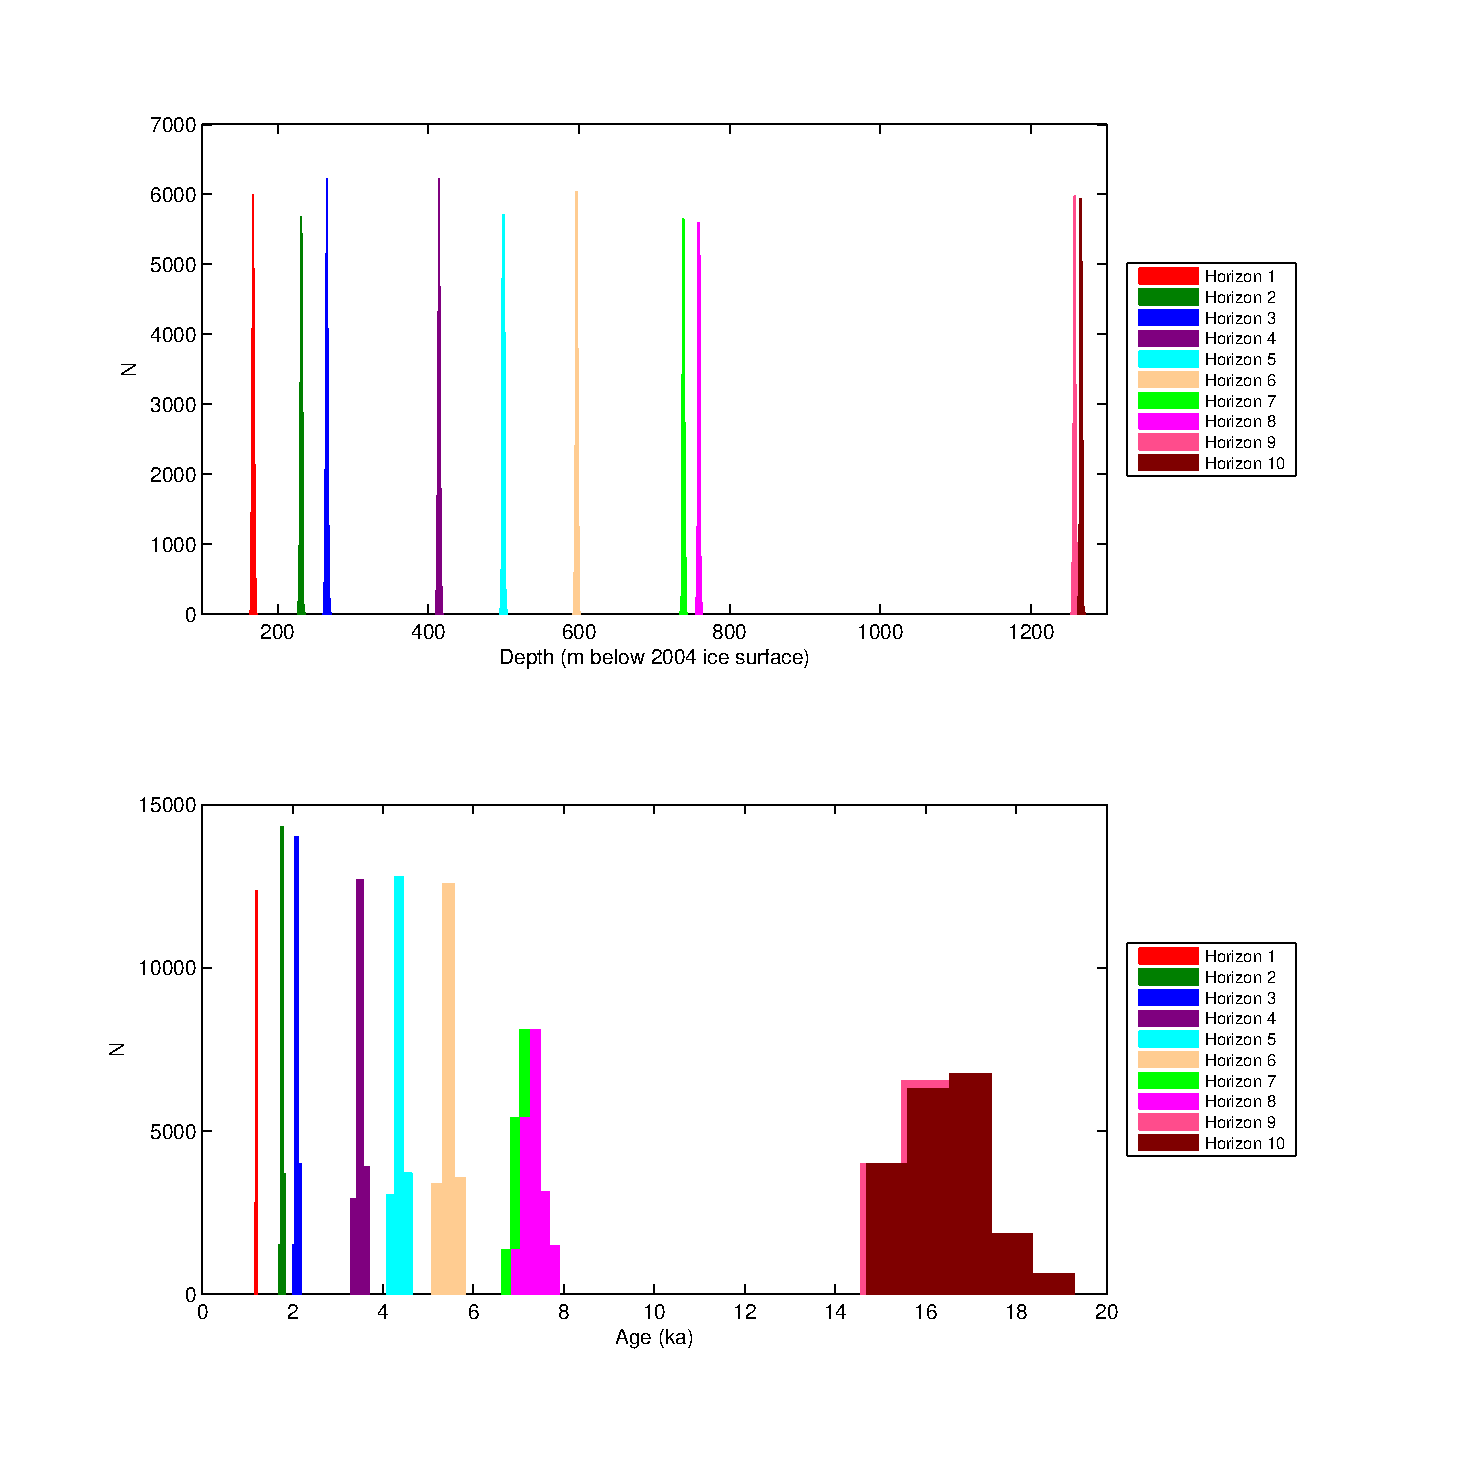
\includegraphics[scale=0.5]{agedepthhist_morland.eps}
\label{agedepthhist}
\captionsetup{width=.9\textwidth}
\caption{a) Histogram of modeled water-equivalent ice depth for each of ten prominent radar horizons observed using airborne radar near Byrd Station, West Antarctica. The width of each distribution is the result of uncertainties arising from the method of radar collection. b) Similar histogram in terms of age (ka). Age uncertainty comes from approximate uncertainty in ice core dating techniques. }
\end{center}
\end{figure}


\begin{figure}
\begin{center}
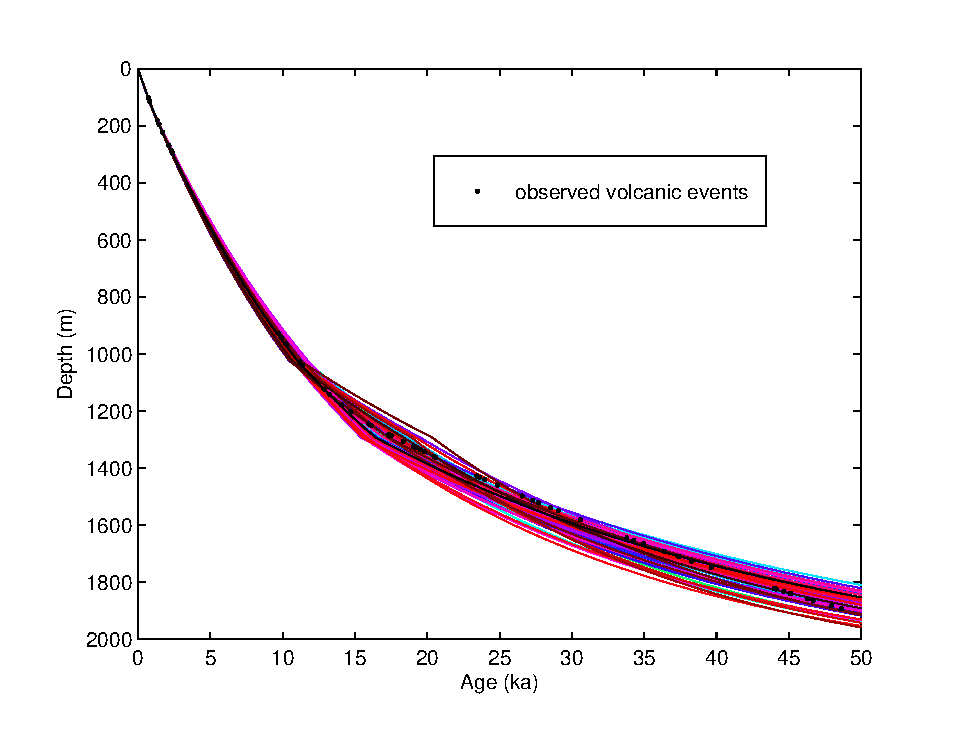
\includegraphics[scale=0.6]{agedepth_metrop.eps}
\label{spaghetti}
\captionsetup{width=.9\textwidth}
\caption{ Ensemble of modeled age-depth profiles near Byrd ice core.  Black dots represent dated volcanic events from the Byrd ice core record \citep{hammer1994}. Each line represents a set of parameters that describe the observed data within uncertainty. (See Section~$\ref{method}$.)   }
\end{center}
\end{figure}

\begin{figure}
\begin{center}
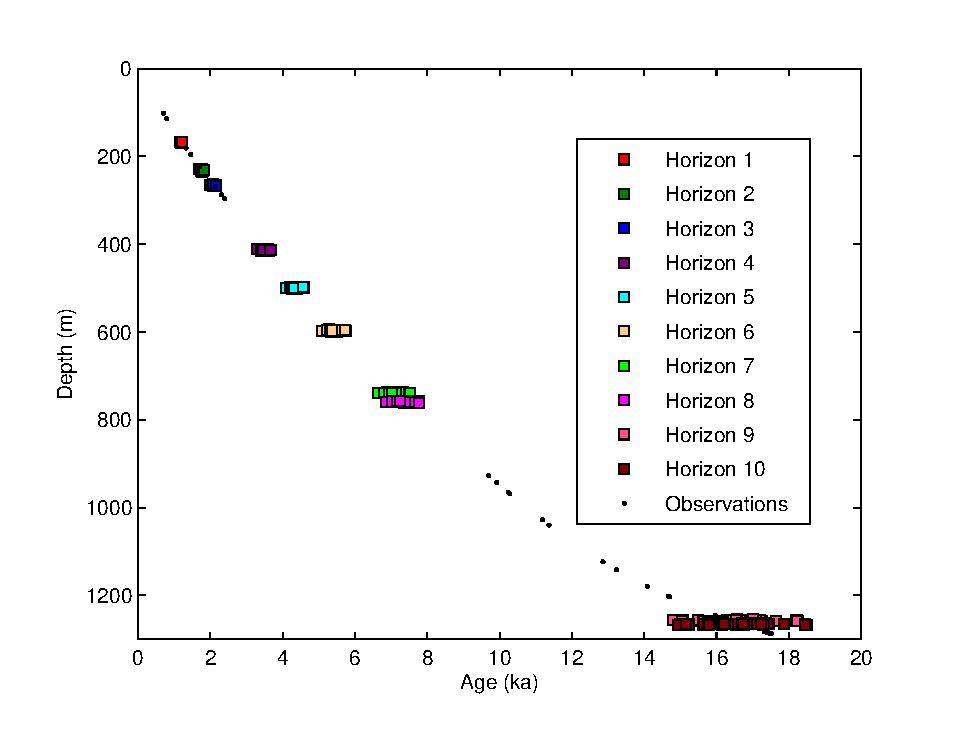
\includegraphics[scale=0.6]{hor_agedepth_morland.eps}
\label{horagedepth}
\captionsetup{width=.9\textwidth}
\caption{ Age-depth profile of ten prominent radar horizons compared to an observed volcanic age-depth profile of the Byrd ice core. The depth and age of each radar horizon are randomly sampled within uncertainty to obtain an ensemble of possible values for that horizon.  }
\end{center}
\end{figure}


\begin{figure}\label{accum}
\begin{center}
%\begin{array}{cc}
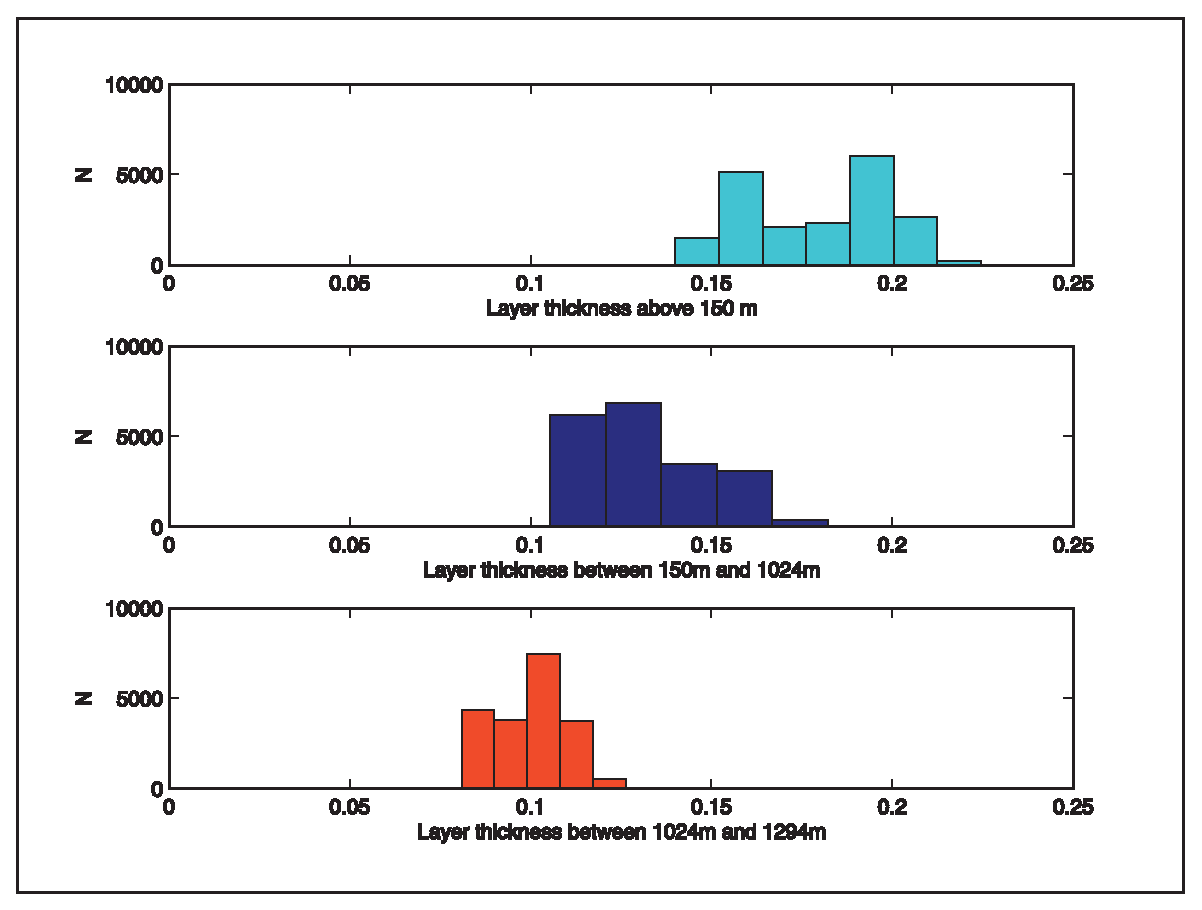
\includegraphics[scale=0.6]{layerthk_v3_10ksamples.eps}
%\end{array}$
\end{center}
\captionsetup{width=.9\textwidth}
\caption{Modeled layer thickness in each of four depth regimes near Byrd Station, West Antarctica. The model overestimates layer thickness, particularly in deeper regimes. }
\end{figure}


\begin{table}\label{accums}
\centering
\begin{tabular}{|c|c|c|}
\hline
Depth Range (m) & \multicolumn{1}{c|}{Layer thickness} & \multicolumn{1}{c|}{Median Layer thickness}  \\
& at Divide (m) & at Byrd  (m)\\
\hline
$\textit{d}$ $<$ 150 & $\sim$ 0.27 &  0.16 $\pm$ 0.04\\
150 $<$ $\textit{d}$ $<$ 1024 & $\sim$ 0.14 - 0.27 & 0.13  $\pm$ 0.06\\
1024 $<$ $\textit{d}$ $<$ 1294 & $\sim$ 0.08 - 0.14 & 0.10 $\pm$ 0.04\\
%$\textit{d}$ $>$ 1294 $<$ &  $\sim$ 0.08 -  0.20 & 0.19 $\pm$ 0.05\\
\hline
\end{tabular}
\captionsetup{width=.9\textwidth}
\caption{Comparison between layer thickness at the Western Divide between the Ross and Amundson Seas \citep{neumann2008} and modeled here at Byrd Station. Maximum layer thickness occurs at the divide, so layer thicknesses at Byrd Station are expected to be less, but comparable, at Byrd Station. We find that layer thickness at Byrd is the same as layer thickness at the Divide to within uncertainty, implying that our model is overestimating layer thickness. This is especially the case at depth, where we expect layer thinning to decrease the thickness of deeper layers due to increased strain. Uncertainties shown are at the 2$\sigma$ level.}
\end{table}

%\begin{table}\label{age_unc}
%\begin{tabular}{|p{4cm}|p{4cm}|p{8cm}|}
%\hline
% Age (a) & 1$\sigma$ Uncertainty (a) & Method of Dating  \\
%\hline
%&&\\
%Age $<$ 1360 & $\pm$ 2  & ECM method on a shallow follow-up ice core, NBY89 from \citep{langway1994}\\
%& & \\
%1360 $\ge$ Age $>$ 11500 & $\pm$ 150  & end of Younger Dryas period and $^{10}Be$ peak ]\citep{blunier1998} \\
%&& \\
%11500 $\ge$ Age $>$ 17320 & $\pm$ 300 & significant volcanic event "Old Faithful" from \citet{hammer1994}\\
%&&\\
%Age $\ge$ 17320 & $\pm$ 2000 & U/Th dating of Laschamp geomagnatic excursion \citep{schramm2000}\\
%\hline
%\end{tabular}
%\captionsetup{width=.9\textwidth}
%\caption{Uncertainty in Byrd ice core chronology Age uncertainty is considered to be gaussian with standard deviation from a variety of age reference points.}
%\tablenotetext{a}{Footnote text here.}
%\end{table}



\begin{table}\label{results}
\centering
\begin{tabular}{| c | c || c | c | c || c | c | c |}
\hline
\multirow{2}{*}{Horizon} & \multicolumn{1}{c||}{TWTT} &  \multicolumn{3}{c||}{Depth (m)} & \multicolumn{3}{c|}{Age (a)} \\   
\cline{3-8}
& ($\mu$s)& Mean & Median & $\sigma$ & Mean & Median & $\sigma$ \\
\hline
 1 & 6.02   & 167.6  & 167.6  & 2.4 & 1200 & 1200 & 20   \\
 2 & 6.78   & 231.4  & 231.4  & 2.4 & 1770 & 1770 & 40   \\
 3 & 7.18   & 265.6  & 265.6  & 2.3 & 2100 & 2100 & 60  \\
 4 & 8.94   & 414.4  & 414.4  & 2.4 & 3510 & 3500 & 150   \\
 5 & 9.94   & 499.6  & 499.6  & 2.4 & 4360 & 4360 & 200   \\
 6 & 11.10  & 596.9  & 596.9  & 2.3 & 5440 & 5440 & 270   \\
 7 & 12.78  & 738.8  & 738.8  & 2.3 & 7120 & 7110 & 370   \\
 8 & 13.02  & 759.1  & 759.1  & 2.3 & 7350 & 7340 & 390   \\
 9 & 18.92  & 1257.7 & 1257.7 & 2.4 & 16220 & 16300 & 1760   \\
 10& 19.02  & 1266.2 & 1266.2 & 2.3 & 16400 & 16500 & 1820  \\
\hline
\end{tabular}
%\tablenotetext{a}{Footnote text here.}
\captionsetup{width=.9\textwidth}
\caption{Depth and age mean, median, and uncertainty for ten strong radar reflectors near Byrd Station, West Antarctica. The radar two-way travel time (TWTT) is given in column 1. }
\end{table}

\end{document}

